\documentclass{article}
\usepackage{../fasy-hw}
\usepackage{ wasysym }
\usepackage{graphicx}

%% UPDATE these variables:
\renewcommand{\hwnum}{2}
\title{Discrete Structures, Homework 1}
\author{Peyton Meeks (Peyton Meeks)}
\collab{n/a}
\date{due: 5 February 2021}

\begin{document}

\maketitle

This homework assignment should be
submitted as a single PDF file both to D2L and to Gradescope.

General homework expectations:
\begin{itemize}
    \item Homework should be typeset using LaTex.
    \item Answers should be in complete sentences and proofread.
    \item You will not plagiarize.  \item List collaborators at the start of each question using the \texttt{collab} command.
    \item Put your answers where the \texttt{todo} command currently is (and
        remove the \texttt{todo}, but not the word \texttt{Answer}).
\end{itemize}

% ============================================
% ============================================
\collab{Luke Cormier} \nextprob{Everyday Mathematical Arguments}
% ============================================
% ============================================
Your sister and you decided to partner on a car washing endeavor, where you
charge cars $\$10$ for a car wash and to split the earnings.  Since you are
doing this at your parents house and they had extra soap, sponges, and a hose
available, there are no costs to you.  At the end of the first day, you have
earned $\$45$ and she had only earned $\$10$. She claimed that you did not pay
her the full payment she deserved. Her argument was: ``If we wash a car, you
earn $\$5$ and I earn $\$5$.  If you earned $\$45$, then we washed nine cars.  If
we wash nine cars, I have earned $\$45$.  I have earned $\$10$; therefore, you
did not give me all of the money that I earned.''  Now, she has not yet taken
Prof.~Fasy's Discrete Structures class, so she does not see the fallacy in her
argument. First, explain which statement that she made that she could not
correctly conclude and explain why.  Second, counter her argument, using
everyday English. The last sentence of your argument should be ``Therefore, I
earned $\$45$ and you earned $\$10$. Third, write this counter argument using
logic statements by first listing the logic statements then writing the argument
mathematically.  Be sure to explain which arguments from Table 2.3.1 that you
are using.

\paragraph{Answer}

She used a converse by saying "If we washed nine cars, I have earned $\$45$. I have earned $\$10$ so you have not payed me. By doing this all she has said was there is a chance that they did not wash nine cars.

If we washed five cars then we made $\$50$. If we made $\$50$ and I made a $\$5$ tip then we made $\$55$. If we made $\$55$ then we should each have $\$27.50$.We washed five cars and I was tipped $\$5$
Therefore, I earned $\$45$ and you earned $\$10$.

Consider the following statements:
\begin{enumerate}
    \item p = ``We earned $\$10$ per carwash''
    \item q = ``We washed 5 cars''
    \item r = ``I was tipped $\$5$"
	\item s = ``We made $\$55$"
\end{enumerate}
If p then qand r therefore s.


% ============================================
% ============================================
\collab{n/a}
\nextprob{Existential Statements}
% ============================================
% ============================================

Are the following statements true or not true?    Prove or disprove.

\begin{enumerate}

    \item All even integers are equal to an odd integer plus one.

        \paragraph{Answer}
        If n is an even interger, then n+1 is a odd integer.
	   0 is an even integer, then 1 is an odd integer.
	   Therefor all even numbers are equal to an odd interger plus one.
	   Modus Ponens

    \item All horses are the same color.

        \paragraph{Answer}
        If one horse is brown, then all horses are brown. This horse is brown, the other horse is black. Therefore not all horses are the same color. Modus Tonens

\end{enumerate}


% ============================================
% ============================================
\collab{n/a}
\nextprob{Division into Cases}
% ============================================
% ============================================

When working at Lockheed Martin, I was invited to play Texas
Hold'em\footnote{For rules, see
here:\url{https://www.pokernews.com/poker-rules/texas-holdem.htm}} at my
colleague's house.  I play with the following rules:
\begin{itemize}
    \item Never fold before the flop.
    \item Never increase the bet.
    \item If it is possible that my hand is \emph{three of a kind} or better,
        match the bet.  Otherwise, fold.
\end{itemize}
My current hand is the jack of hearts and the 10 of diamonds, and the flop is 10
of hearts, 3 of clubs, and king of hearts.

\begin{enumerate}

    \item What are the cases that could occur for the Turn card?  What is the
        outcome (match or fold) for these different cases? (Note: rather than
        listing every possible card, try to categorize the cards into as few
        classes as possible).

    \paragraph{Answer}
    Case 1: Another 10, Match Bet
	Case 2: Any other card, Fold

    \item Suppose that the Turn card is the jack of clubs.
        What are the cases that could occur for the River card, and what is the
        outcome (match or fold) for these different cases?  (Again, try to
        describe this in as few cases as possible).

    \paragraph{Answer}
    Case 1: Another 10 or Jack, Match Bet
	Case 2: Any other card, Fold

\end{enumerate}


% ============================================
% ============================================
\collab{n/a}
\nextprob{Bipartite Graphs}
% ============================================
% ============================================

Exercise Set 4.9, Question 23.

\paragraph{Answer}
\begin{itemize}

	\item A.
		\begin{figure}[h]
		\centering
			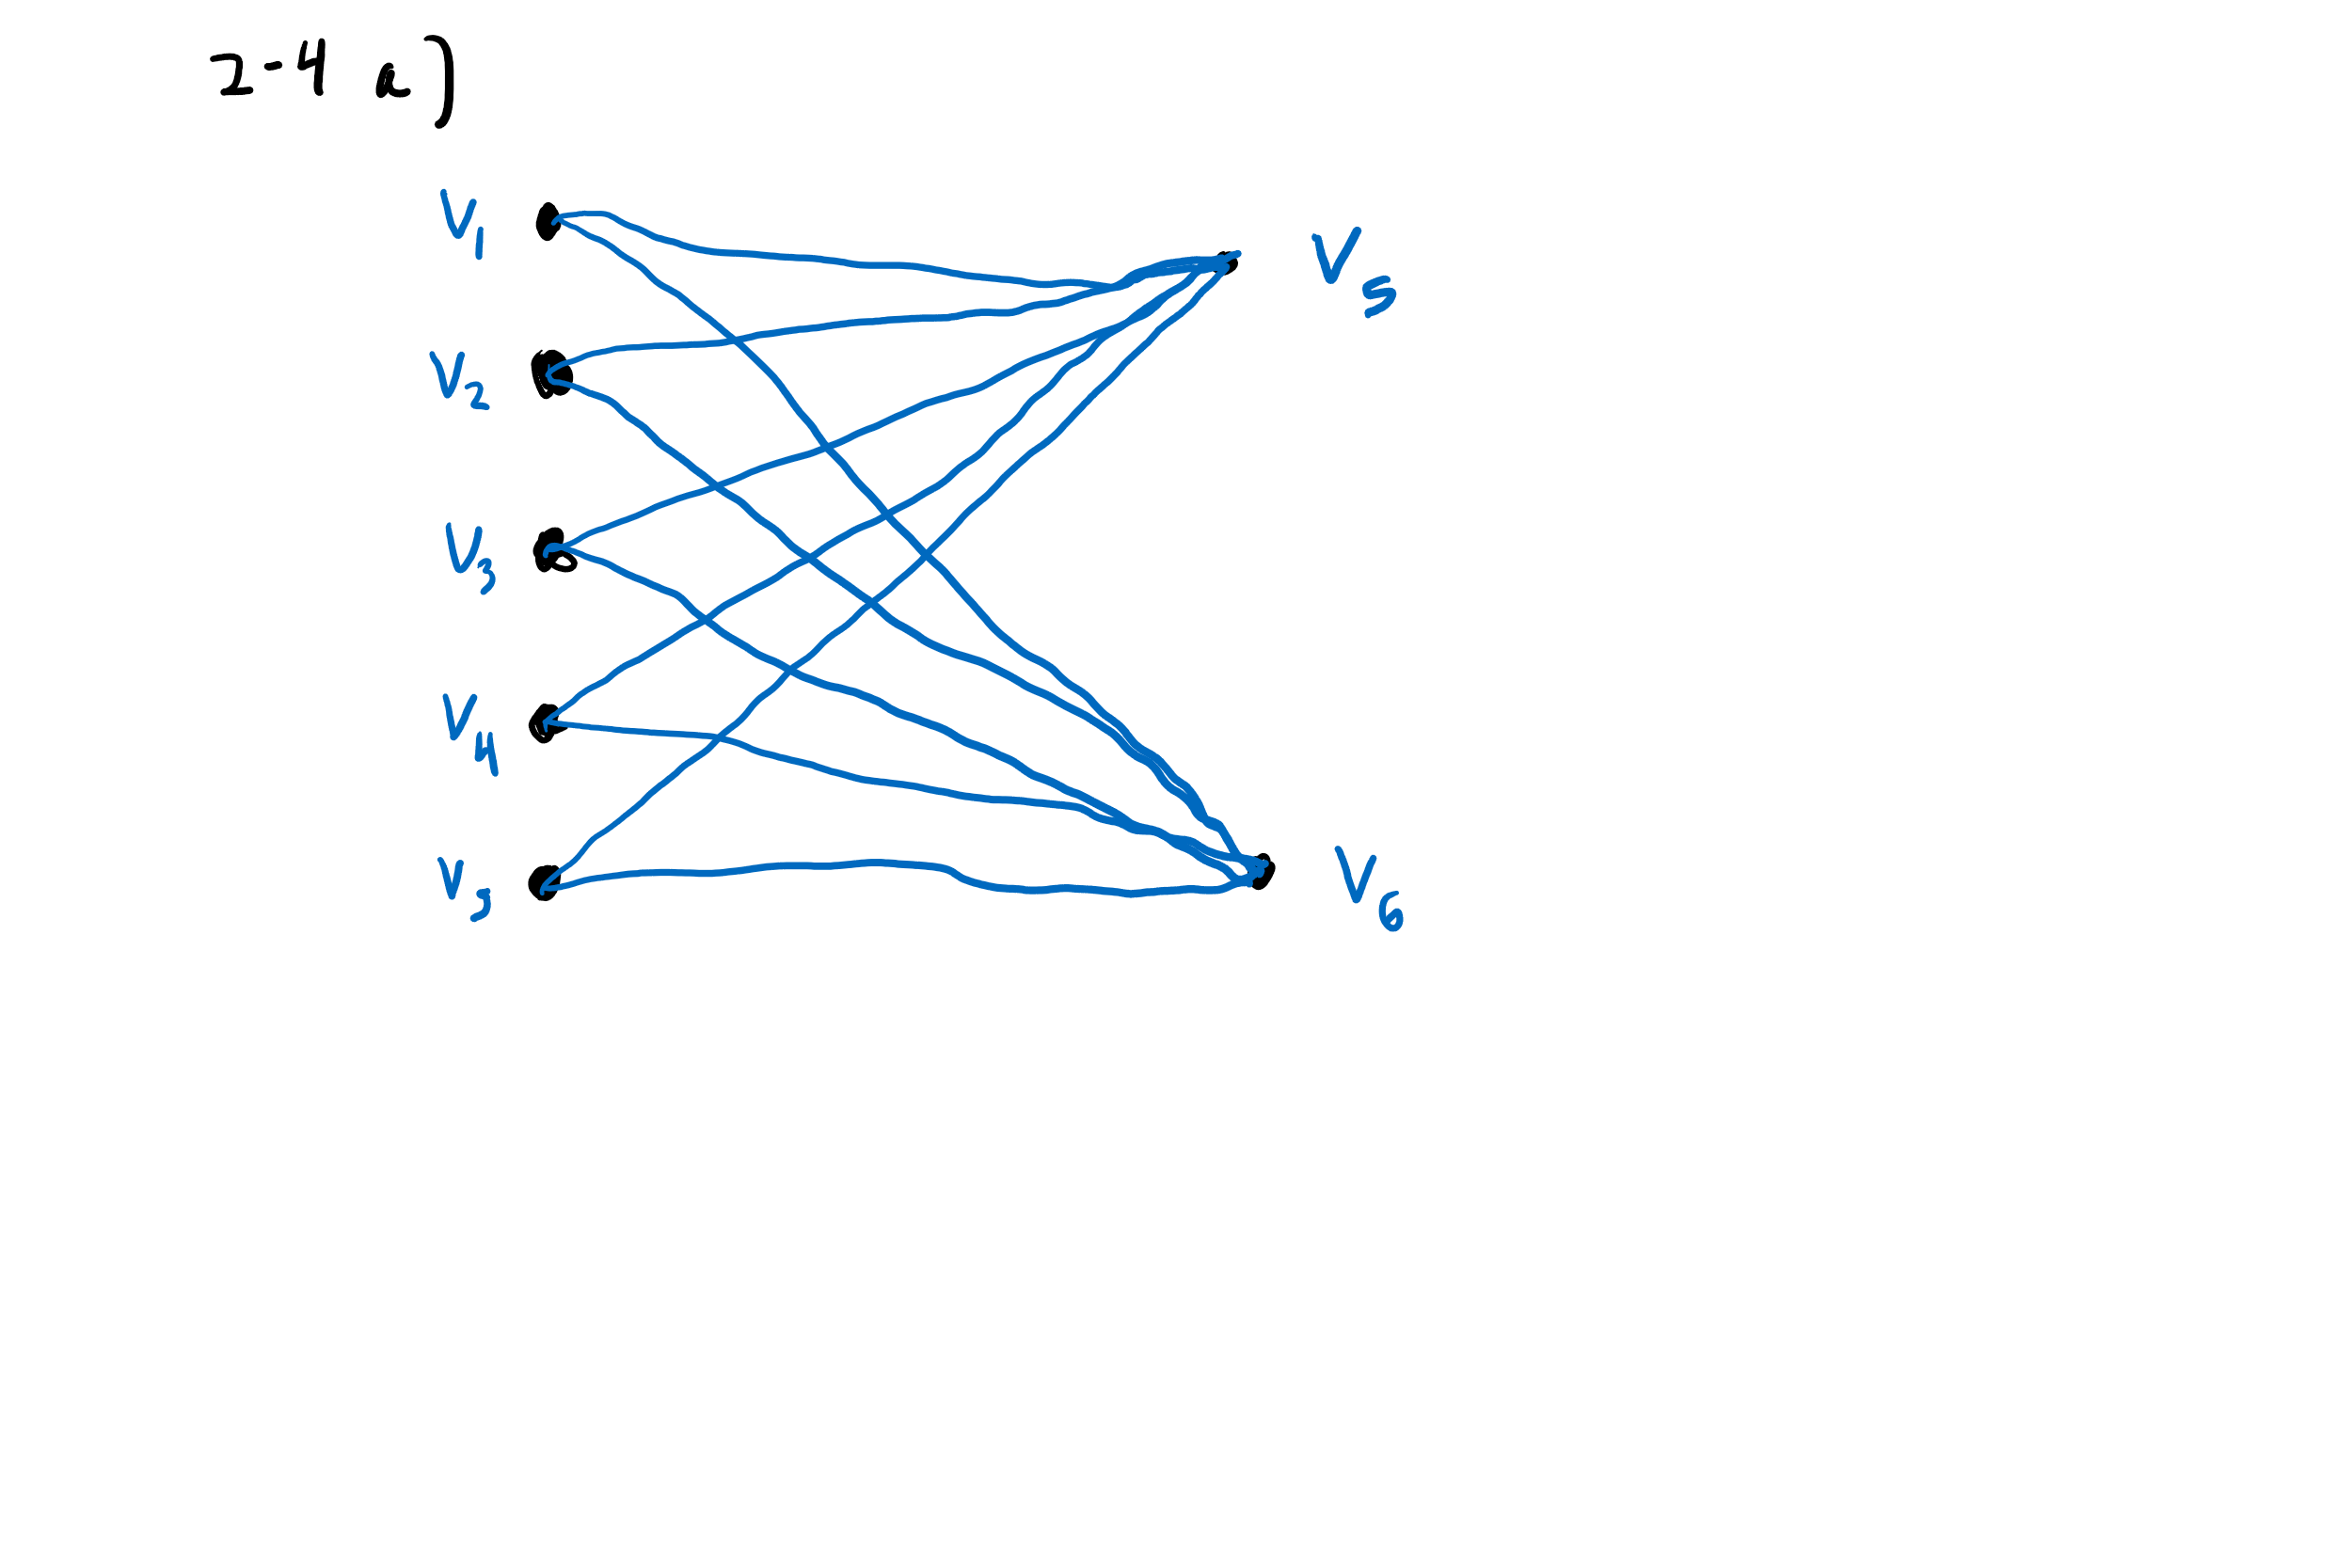
\includegraphics[width=0.25\textwidth]{H_2-4_a}
		\end{figure}

	\item B.
		\begin{figure}[h]
		\centering
			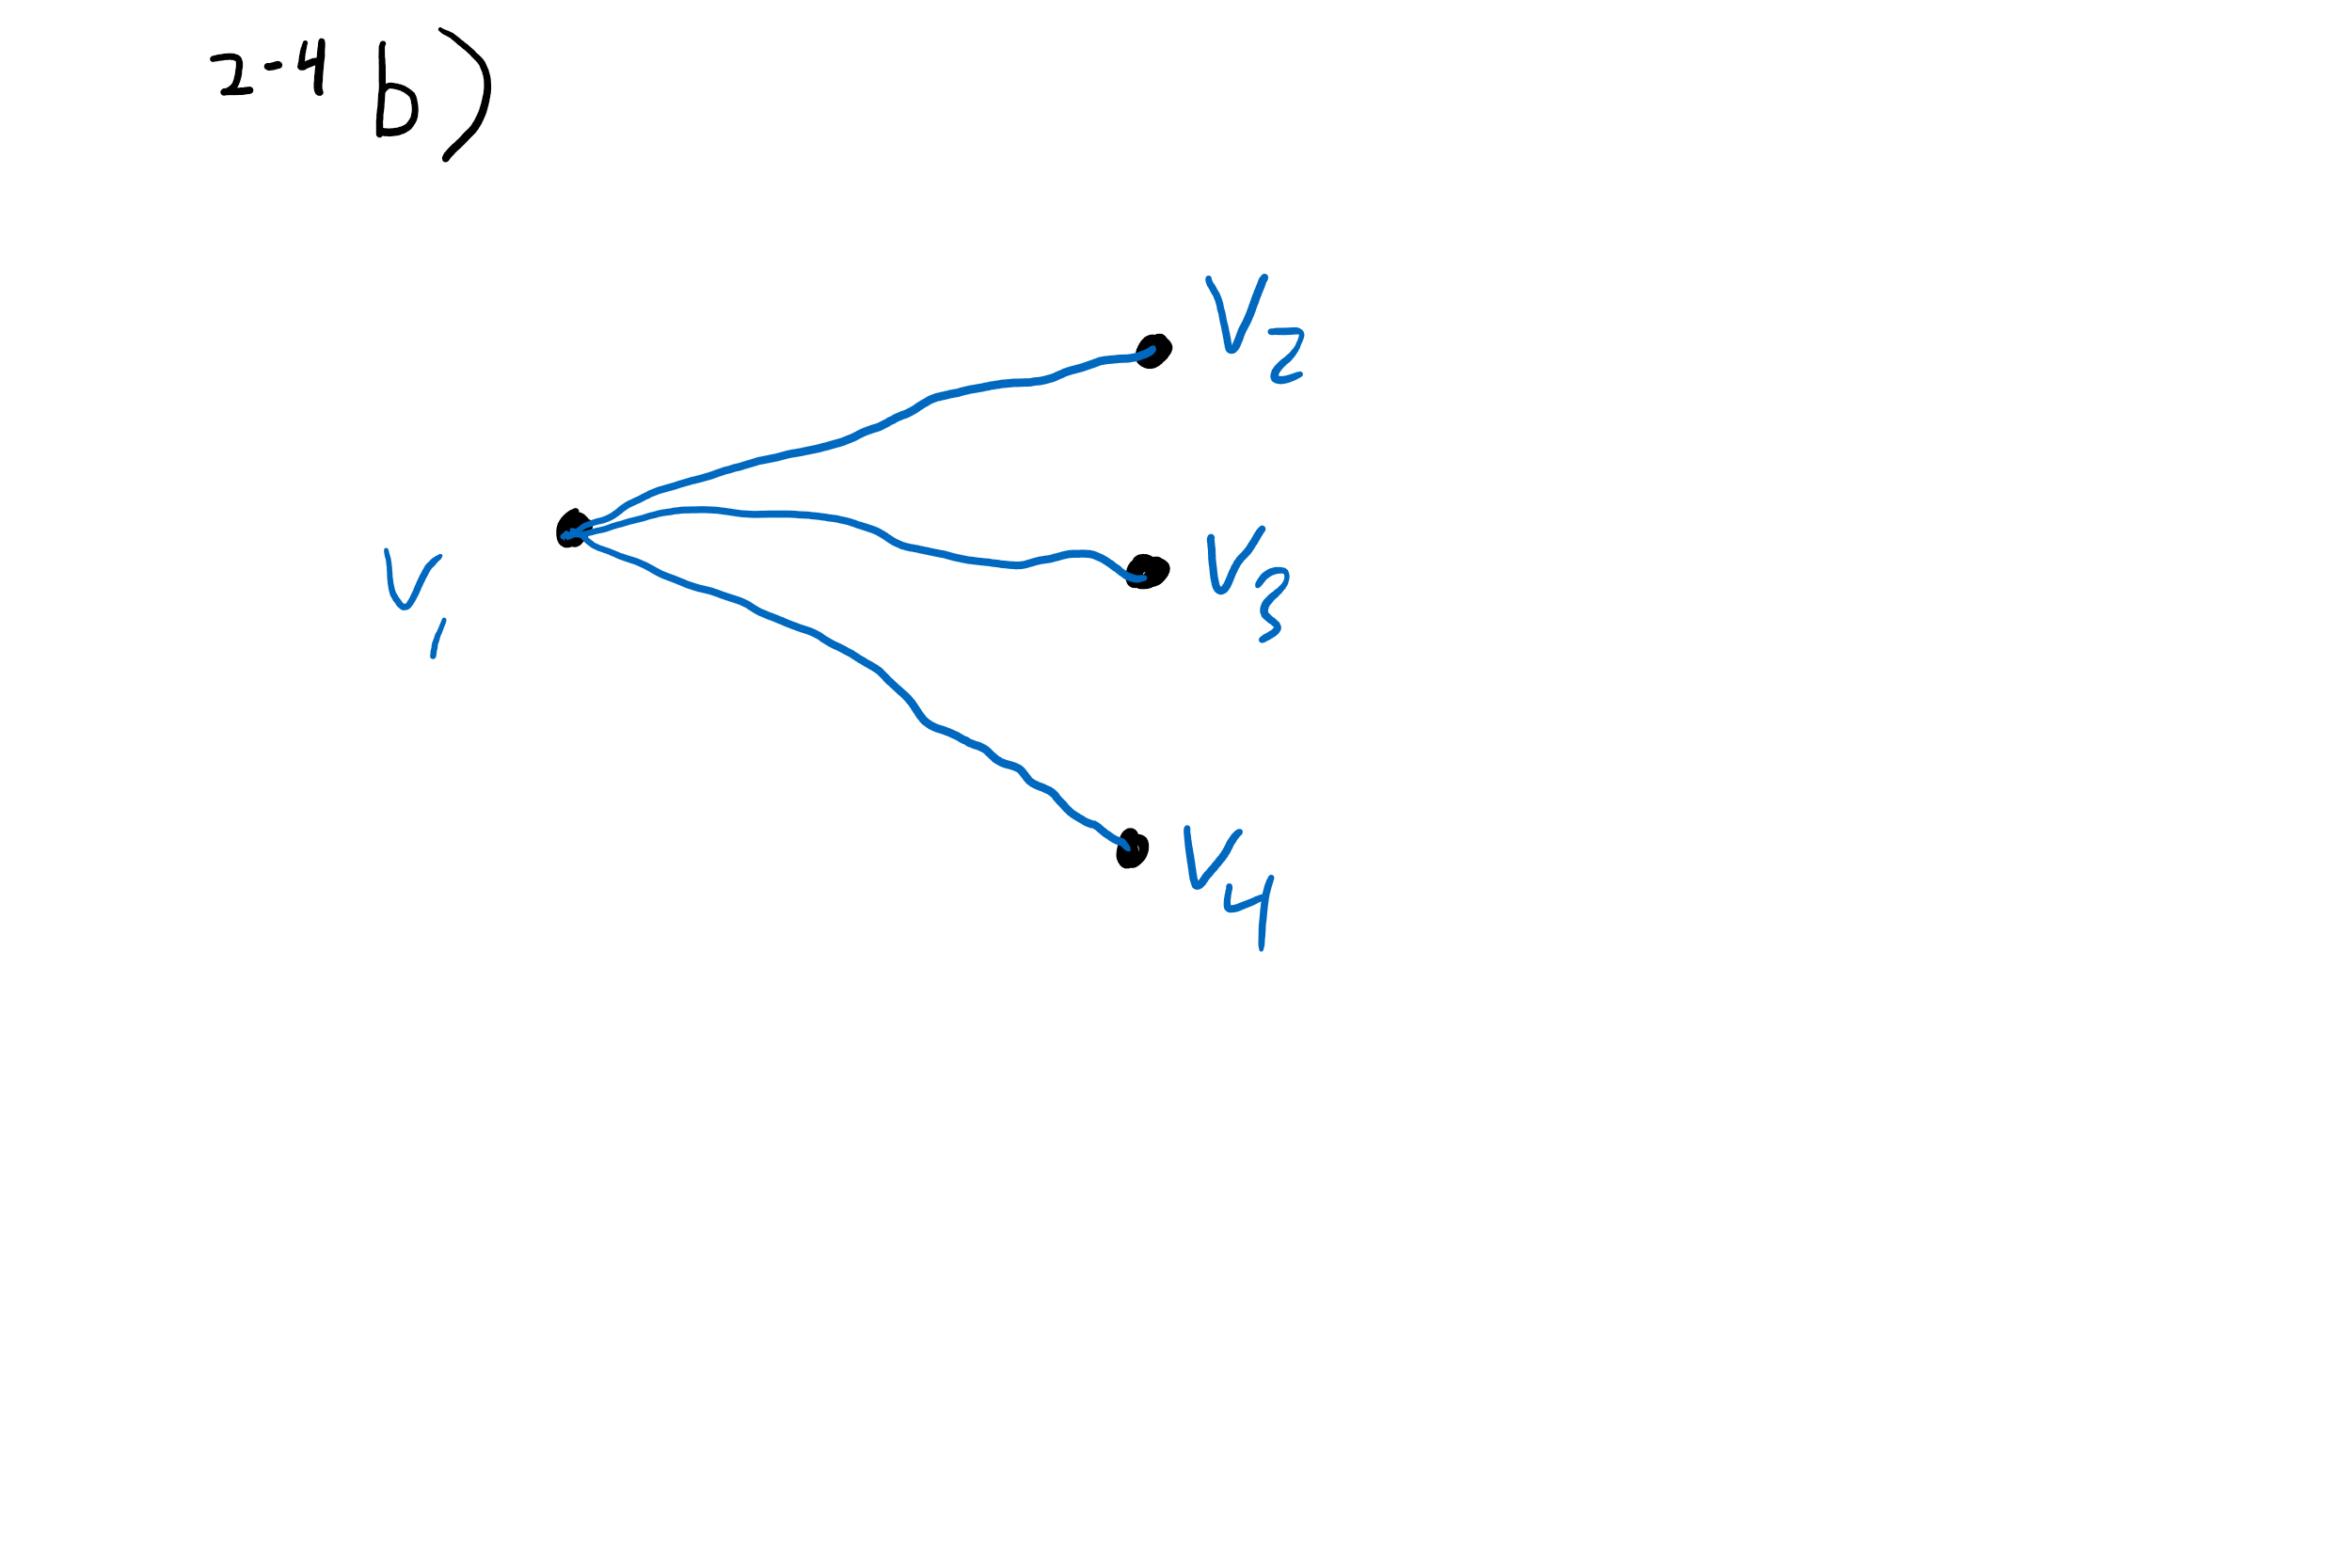
\includegraphics[width=0.25\textwidth]{H_2-4_b}
		\end{figure}	

	\item C.
		\begin{figure}[h]
		\centering
			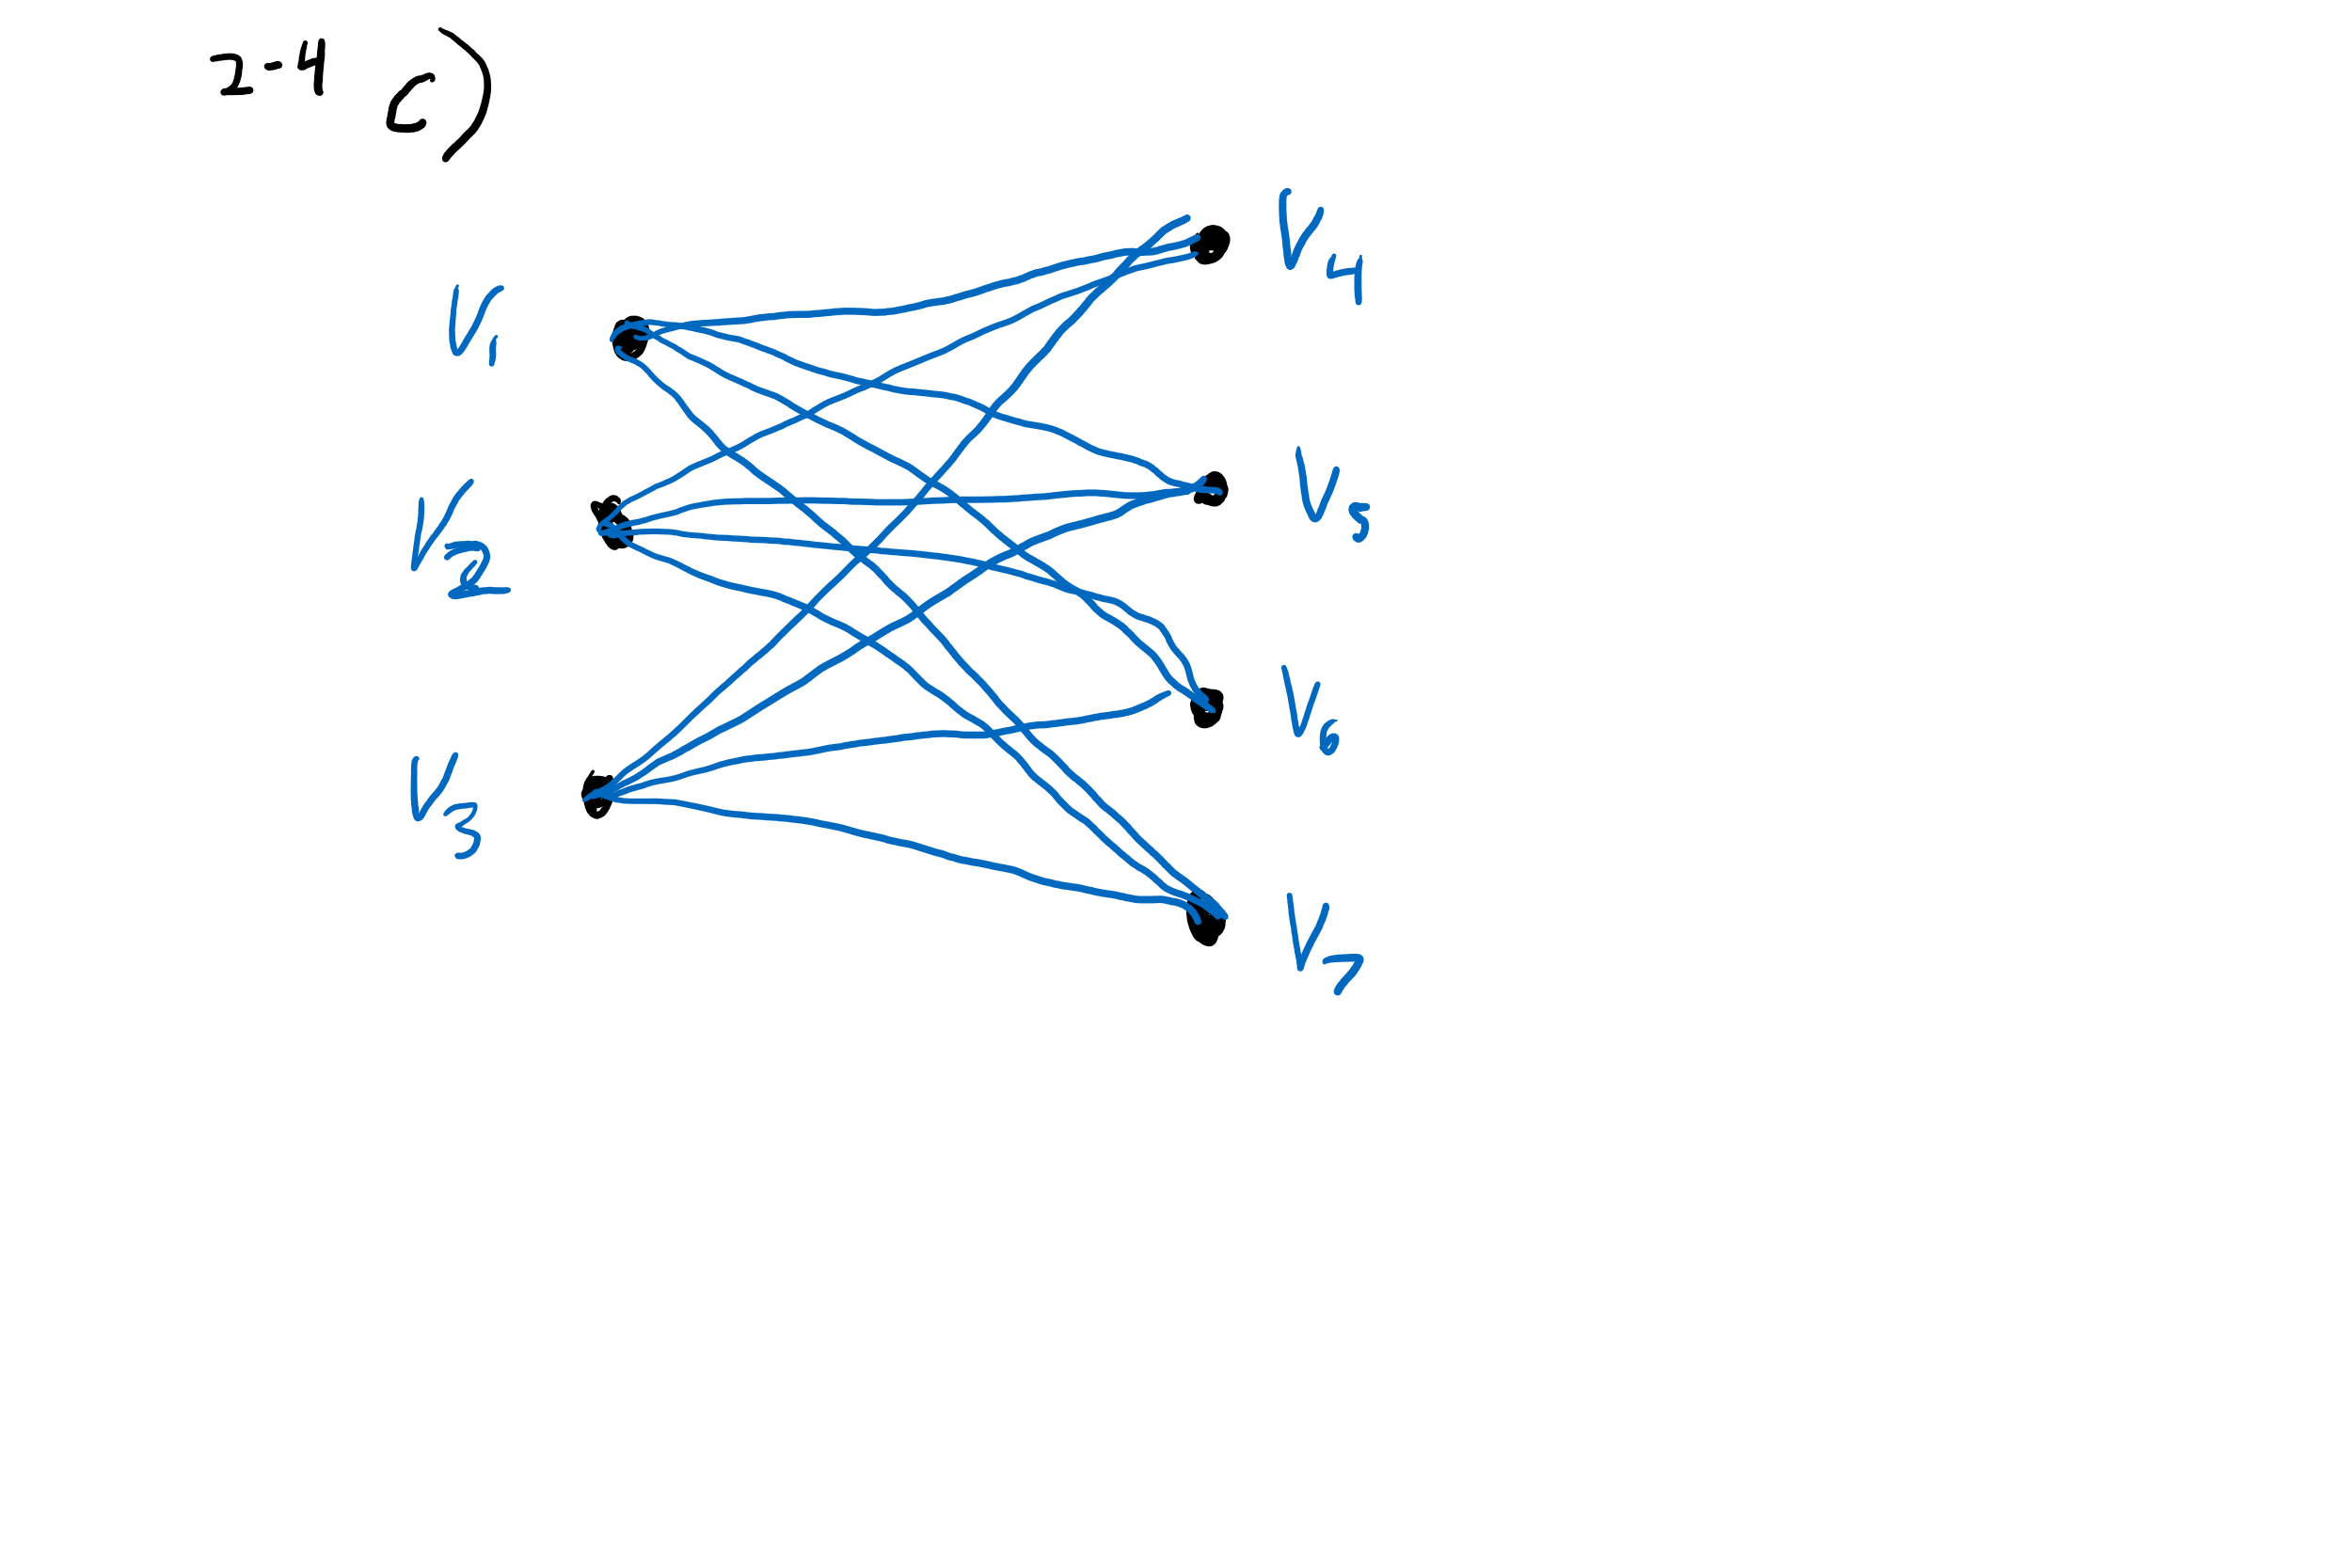
\includegraphics[width=0.25\textwidth]{H_2-4_c}
		\end{figure}

	\item D.
		All vertices in group of size m have degree n, all vertices of group size n have degree m.

	\item E.
		m+n
	\item F.
		m*n


\end{itemize}

% ============================================
% ============================================
\collab{n/a}
\nextprob{Four Color Theorem}
% ============================================
% ============================================
Read Chapter 1 of \emph{Four Colors Suffice} and answer the following questions:

\begin{enumerate}

    \item Consider the map of the continental US on Page 5.  Why can we color
        Utah and New Mexico the same color, even though the two states touch at
        a point?

        \paragraph{Answer}
        Since they only touch at a single point they can be colored the same.

    \item Again, looking at the map of the continental US on Page 5, explain why
        Michigan does not satisfy the conditions for the four color theorem.

        \paragraph{Answer}
        Michigan is only touching three other states but they are not neighboring.

    \item Explain why we an omit the states of Hawaii and Alaska in order to
        construct a four-coloring of the states in the USA.

        \paragraph{Answer}
        Since they are not conjoined to the continental US in anyway they must be omitted.

    \item Is the following statement TRUE or FALSE?  Explain. Four colors are
        necessary to color all maps.

        \paragraph{Answer}
        False, if there are not many area's to be covered then less then four colors will do.

    \item Explain one application of the four color theorem that does not
        involve coloring geographic maps.

        \paragraph{Answer}
        A jigsaw puzzle
    \item (Extra Credit). Provide a four-coloring of the McGregor April Fool's
        Hoax on Page 11.

        \paragraph{Answer}
        \todo{Your answer here; should include a figure}

\end{enumerate}

% ============================================
% ============================================
\collab{n/a}
\nextprob{Fred Brooks}
% ============================================
% ============================================

Write a short (1-2 paragraph) biography of Fred Brooks.  He wrote the book
entitled \emph{The Mythical Man Month}~\cite{brooks-manmonth}.  In your
biography, explain what the title of this book means.
\textbf{In your own words}, describe who they are and why they are important in
the history of computer science.  If you use external resources, please provide
proper citations. If you do not use external sources, please write ``I did not
use any sources to write this biography'' as the last sentence of the
biography.

\paragraph{Answer}
	\paragraph{
Fred Brooks was one of the nations foremost computer scientists, even before computer science was called computer science. He used his time at The University of Harvard to study automatic data processing. From there he joined IBM working on some of the most impressive computers of the time. One of which was used at the NSA. Later he returned to his home state of North Carolina to found UNC's computer science department. He spent most of his years there continuing reaserch on various projects which have influced computer science in many ways. After leaving IBM, Brooks wrote his infamous book \emph{The Mythical Man Month}~\cite{brooks-manmonth}. This book talked aobut the sucess and struggles Brooks experienced during his software engineering days at IBM.}


%% ... the bibliography
\newpage
\bibliographystyle{acm}
\bibliography{biblio}
\begin{itemize}
	\item \url{https://en.wikipedia.org/wiki/Fred_Brooks}
\end{itemize}

\end{document}

